\documentclass[12pt]{article}
\usepackage{enumerate}
\usepackage{amsmath}
\usepackage{amsthm}
\usepackage{amssymb}
\usepackage{changepage}\usepackage{graphicx}

\title{Assignment 2}
\author{Rin Meng \\ Student ID: 51940633}

\begin{document}
\maketitle

\begin{enumerate}[1.]
    \item Given the summary output, it is true that:
    \begin{enumerate}[(a)]
        \item \[\text{F-Statistic} = 52.77\]
        \[\text{MSE} = (\text{Residual Standard Error})^2 = 2.792^2 =  7.80\]
        \item To build the anova table, we need to do calculations as follows:
        
            Finding the degrees of freedom:
            \[ DF_{Reg} = 1 \]
            \[ DF_{Error} = 7 \]
            \[ DF_{Total} = 8 \]
            \[ SS_{Total} = SS_{Reg} + SS_{Error}\]
            Calculate the Mean Squares Reg and Error:
            \[ F = \frac{MS_{Reg}}{MS_{Error}} = 52.77\]
            \[ MS_{Error} = MSE = 7.80\]
            \[ MS_{Reg} = F \cdot MS_{Error} = 52.77 \cdot 7.80 = 411.34\]
            Calculate the Sum Squares Reg and Error:
            \[ MS_{Reg} = \frac{SS_{Reg}}{DF_{Reg}} \Leftrightarrow SS_{Reg} = MS_{Reg} \cdot DF_{Reg}\]
            \[ MS_{Error} = \frac{SS_{Error}}{DF_{Error}} \Leftrightarrow SS_{Error} = MS_{Error} \cdot DF_{Error}\]
            \[ SS_{Total} = SS_{Reg} + SS_{Error}\]
            \[ SS_{Reg} = MS_{Reg} \cdot DF_{Reg} = 411.34 \cdot 1 = 411.34\]
            \[ SS_{Error} = MS_{Error} \cdot DF_{Error}= 7.80 \cdot 7 = 54.60 \]
            \[ SS_{Total} = SS_{Reg} + SS_{Error} = 411.34 + 54.60 = 465.94\]
            \[ MS_{Total} = \frac{SS_{Total}}{DF_{Total}} = \frac{465.94}{8} = 58.24 \]
            \begin{center}
                \begin{tabular}{|c|c|c|c|c|}
                    \hline
                    Source & DF & SS & MS & F \\
                    \hline
                    Reg. & 1 & 411.34 & 411.34 & 52.77 \\
                    Error & 7 & 54.60 & 7.80 &  \\
                    Total & 8 & 465.94 & 58.24 & \\
                    \hline
                \end{tabular}
            \end{center}
        \item The anova function returns:
            \begin{verbatim}
Analysis of Variance Table

Response: R
        Df Sum Sq Mean Sq F value    Pr(>F)    
W          1 411.42  411.42  52.767 0.0001679 ***
Residuals  7  54.58    7.80                      
---
Signif. codes:  0 ‘***’ 0.001 ‘**’ 0.01 ‘*’ 0.05 ‘.’ 0.1 ‘ ’ 1
            \end{verbatim}
            Our hand calculations are fairly consistent with the output from the anova
            function in R, minus a few rounding errors.
        \item Calculating the $\sqrt{F}$ value:
            \[ \sqrt{F} = \sqrt{52.77} = 7.27 \]
            The t value for $\hat{\beta}_1$ is 7.264, which is very close to the $\sqrt{F}$ 
            value. This is expected because, for simple linear regression with one 
            predictor, the square of the t-value for the slope is equal to the 
            F-statistic 
            \[ \sqrt{F} = t \Leftrightarrow F = t^2 \]
    \end{enumerate}
    
    \item Given
        \begin{enumerate}
            \item 
                \begin{enumerate}[-]
                    \item \textbf{First task time}: $\epsilon$ is 
                    exponentially distributed with mean $ \frac{1}{\lambda} $, so $E[\epsilon] = \frac{1}{\lambda}$.
                    \item \textbf{Second task time}: Proportional to $x$, with a proportionality constant $\beta$. So the time required 
                    should be $\beta x$.
                    \item \textbf{Total time}: sum of times it takes to complete the two tasks
                    impying that the total time is $y = \beta x + \epsilon$.
                \end{enumerate}
            
                Then the final linear model would be 
                \[y = \beta x + \epsilon \]

            \item To derive the maximum likelihood estimator for $\beta$ and $\lambda$, we need to find the pdf of the exponential distribution.
                \[f(\epsilon) = \lambda e^{-\lambda \epsilon} \text{ for } x \geq 0\]
                \[\Rightarrow f(y) = \lambda e^{-\lambda (y - \beta x)} \text{ for } y \geq \beta x\]

                Deriving maximum likelihood estimator for $\beta$:
                \begin{align*}
                    L(\beta, \lambda) &= \prod_{i=1}^{n} \lambda e^{-\lambda (y_i - \beta x_i)} \\
                    \log (\beta, \lambda) &= \ell (\beta, \lambda) = \sum_{i=1}^{n} \log (\lambda e^{-\lambda (y_i - \beta x_i)}) \\
                    \frac{\partial \ell (\beta, \lambda)}{\partial \beta} &= \sum_{i=1}^{n} \frac{\partial}{\partial \beta} \left( \log (\lambda e^{-\lambda (y_i - \beta x_i)}) \right) \\
                    \frac{\partial \ell (\beta, \lambda)}{\partial \beta} &= \sum_{i=1}^{n} \frac{\partial}{\partial \beta} \left( \log \lambda - \lambda (y_i - \beta x_i)  \right) \\
                    \frac{\partial \ell (\beta, \lambda)}{\partial \beta} &= \sum_{i=1}^{n} -x_i \lambda + x_i \lambda \beta \\
                    \frac{\partial \ell (\beta, \lambda)}{\partial \beta} &= \sum_{i=1}^{n} -x_i \lambda + x_i \lambda \beta = 0 \\
                    \sum_{i=1}^{n} x_i \lambda &= \sum_{i=1}^{n} x_i \lambda \beta \\
                    \beta &= 1
                \end{align*}
                Deriving maximum likelihood estimator for $\lambda$:
                \begin{align*}
                    L(\beta, \lambda) &= \prod_{i=1}^{n} \lambda e^{-\lambda (y_i - \beta x_i)} \\
                    \log L(\beta, \lambda) &= \ell (\beta, \lambda) = \sum_{i=1}^{n} \log \lambda e^{-\lambda (y_i - \beta x_i)} \\
                    \frac{\partial \ell (\beta, \lambda)}{\partial \lambda} &= \sum_{i=1}^{n} \frac{\partial}{\partial \lambda} \left(  \log \lambda e^{-\lambda (y_i - \beta x_i)} \right) \\
                    \frac{\partial \ell (\beta, \lambda)}{\partial \lambda} &= \sum_{i=1}^{n} \frac{\partial}{\partial \lambda} \left( \log \lambda - \lambda (y_i - \beta x_i) \right) \\
                    \frac{\partial \ell (\beta, \lambda)}{\partial \lambda} &= \sum_{i=1}^{n} \frac{1}{\lambda} - (y_i - \beta x_i) \\
                    \frac{\partial \ell (\beta, \lambda)}{\partial \lambda} &= \sum_{i=1}^{n} \frac{1}{\lambda} - (y_i - \beta x_i) = 0 \\
                    \sum_{i=1}^{n} \frac{1}{\lambda} &= \sum_{i=1}^{n} (y_i - \beta x_i) \\
                    \frac{n}{\lambda} &= \sum_{i=1}^{n} (y_i - \beta x_i) \\
                    \lambda &= \frac{n}{\sum_{i=1}^{n} (y_i - \beta x_i)}
                \end{align*}

                $\therefore$ The maximum likelihood estimator for $\beta$ is 1 and $\lambda$ is $\frac{n}{\sum_{i=1}^{n} (y_i - \beta x_i)}$.
                
            \item 
            
            Summary function returns:
            \begin{verbatim}
Call:
lm(formula = y ~ 0 + x, data = data)

Residuals:
     Min       1Q   Median       3Q      Max 
-0.58177  0.01169  0.30713  0.50050  1.64693 

Coefficients:
  Estimate Std. Error t value Pr(>|t|)    
x   1.2653     0.1389   9.111 7.72e-06 ***
---
Signif. codes:  0 ‘***’ 0.001 ‘**’ 0.01 ‘*’ 0.05 ‘.’ 0.1 ‘ ’ 1

Residual standard error: 0.7179 on 9 degrees of freedom
Multiple R-squared:  0.9022,	Adjusted R-squared:  0.8913 
F-statistic:    83 on 1 and 9 DF,  p-value: 7.725e-06
            \end{verbatim}
            \item To plot the scatter plot, we can run this code:
            \begin{verbatim}
plot(data$x, data$y, main = "Scatterplot with Fitted Line",
 xlab = "x", ylab = "y", pch = 19)
abline(model, col = "red")
            \end{verbatim}
            
            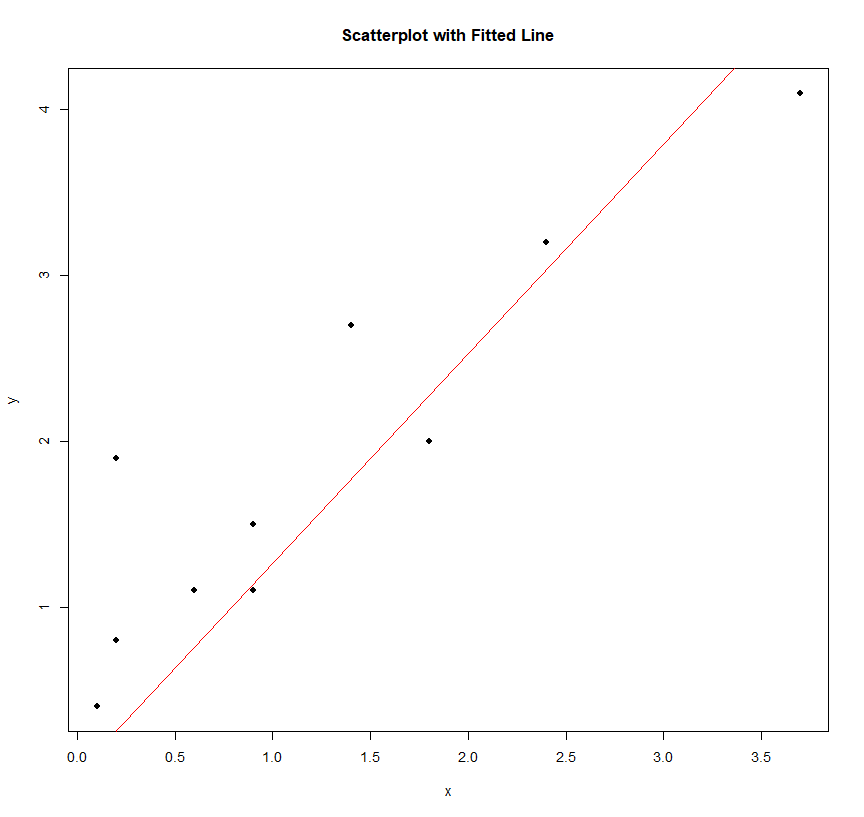
\includegraphics[width=0.80\textwidth]{Rplot.png}

            \item We can calculate the residuals using the equation $e_i = y_i - \hat{y}_i $ or the function 
            \begin{verbatim}
residuals(model)
            \end{verbatim}

            Which will return
            \begin{verbatim}
          1           2           3           4           5
-0.27761976  0.27346557  1.64693114  0.92851796  0.16317365
          6           7           8           9          10
-0.03880988  0.36119012  0.34079341  0.54693114 -0.58177395 
            \end{verbatim}

            and the mean of the residuals is $0.336$.

            Comments:

            \begin{enumerate}
                \item The residuals are not centered around 0 since the mean is 0.336, that means the model may not be a good fit.
                \item The residuals does not seem to be symmetrically distributed around 0 (there are more positives than negatives), 
                therefore, the assumption of normality is not satisfied.
            \end{enumerate}

            \item The OLS being used to fit would be biased in this case because:
            \begin{enumerate}
                \item The error term $\epsilon$ is not centered at zero (exponential distribution is always positive)
                \item Key assumtion that $E[\epsilon] = 0$ but it's actually $E[\epsilon] = \frac{1}{\lambda}$
                \item For all $\epsilon$, it would be expoentially distributed
            \end{enumerate}

            For the model, we can express the expected value of y, 
            \[ E[y] = E[\beta x + \epsilon] = \beta x + E[\epsilon]  = \beta x + \frac{1}{\lambda}\]
            Here, we reap what we sow. When we apply OLS to the model, we will be making an assumtion that $E[\epsilon] = 0$,
            and we can see that OLS will be estimating $\beta$ biased towards $\frac{1}{\lambda}$ which would be $E[\epsilon] = 0.336$.
            
            \item For the least-squares estimate of $\beta$, to be unbiased, assuming the regression through the origin model,
            the condition required should be that
            \begin{enumerate}
                \item The error term $\epsilon$ is centered at 0
                \item $Cov(x, \epsilon) = 0$
                \item The error term $\epsilon$ is normally distributed
            \end{enumerate}
            Withholding these conditions, the OLS estimate of $\beta$ will be unbiased.
        \end{enumerate}

        \item Ploting the data, we can run this code:
            \begin{enumerate}
                \item 
                \begin{verbatim}
# Define the vectors for angle and distance
angle <- c(1.3, 4.0, 2.7, 2.2, 3.6,
             4.9, 0.9, 1.1, 3.1)
distance <- c(0.43, 0.84, 0.58, 0.58, 
            0.70, 1.00, 0.27, 0.29, 0.63)
plot(angle, distance,
        xlab = "Angle of Ramp (degrees)", 
        ylab = "Distance Travelled (m)",
        main = "Distance Travelled by Angle of Ramp", 
        pch = 19, col = "blue")
                \end{verbatim}
                Which will return
            
            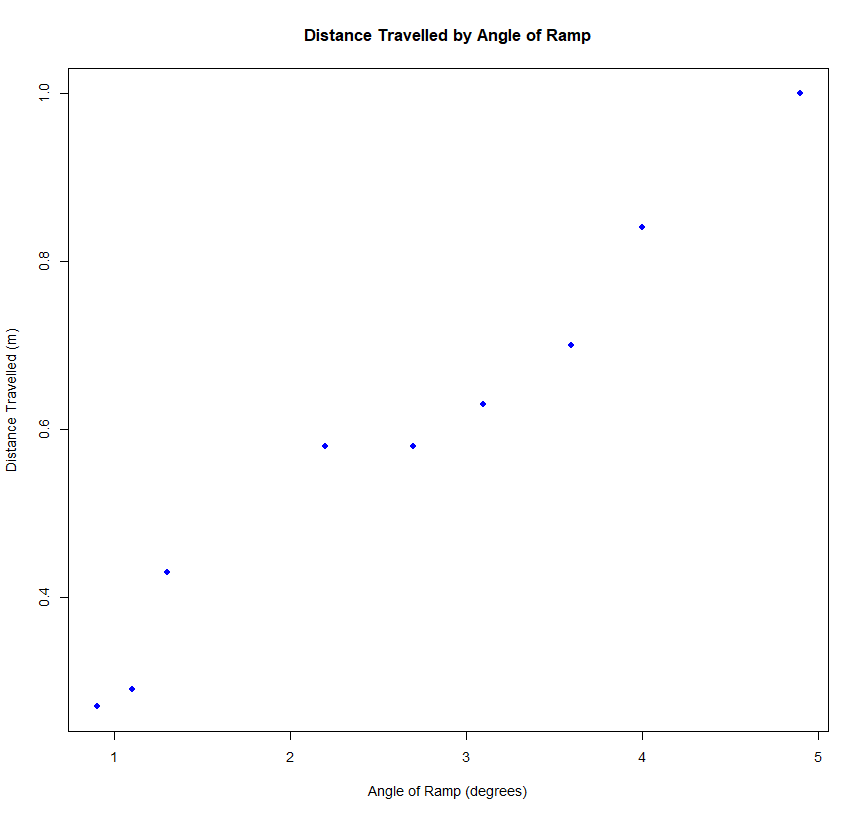
\includegraphics[width=0.70\textwidth]{Rplot02.png}

            Where angle is our predictor $y$ (angle), and distance is our response $x$ (distance).

            Is a linear model reasonable?
            \begin{enumerate}
                \item On physical grounds, we know that a steep ramp angle could result in higher gravitational component acting
                along the ramp, so we would expect some increase in the distance travelled, but should not be perfectly linear
                becauuse of other factors like friction, air resistance, etc.
                \item On statistical grounds, the since the points are not perfectly linear (noticable curve and dispersion),
                we can say that the relationship between the angle of the ramp and the distance travelled is not linear, therefore
                suggesting that a linear model may not be the best fit.
            \end{enumerate}

            \item Now we compute, the slope and intercept for the linear model, i.e $S_{xx}$, $S_{xy}$, 
            $\bar{y}$, $\bar{x}$.
            First we recall that
            \begin{enumerate}
                \item $\bar{x} = \frac{1}{n} \sum_{i=1}^{n} x_i$
                \item $\bar{y} = \frac{1}{n} \sum_{i=1}^{n} y_i$
                \item $S_{xx} = \sum_{i=1}^{n} (x_i - \bar{x})^2$
                \item $S_{xy} = \sum_{i=1}^{n} (x_i - \bar{x})(y_i - \bar{y})$
                \item $\hat{\beta}_1 = \frac{S_{xy}}{S_{xx}}$
                \item $\hat{\beta}_0 = \bar{y} - \hat{\beta}_1 \bar{x}$
            \end{enumerate}
            Now we can calculate the values:
            \[ \bar{x} = \frac{23.8}{9} = 2.64 \]
            \[\bar{y} = \frac{5.32}{9} = 0.59 \]
            \begin{align*}
                S_{xx} &= (1.3-2.64)^{2}+(4.0-2.64)^{2}+(2.7-2.64)^{2}\\
                &+(2.2-2.64)^{2}+(3.6-2.64)^{2}+(4.9-2.64)^{2}\\
                &+(0.9-2.64)^{2}+(1.1-2.64)^{2}+(3.1-2.64)^{s2} \\
                &= 15.48
            \end{align*}
            \begin{align*}
                S_{xy} &= (1.3-2.64)(0.43-0.59)+(4.0-2.64)(0.84-0.59)\\
                &+(2.7-2.64)(0.58-0.59)+(2.2-2.64)(0.58-0.59)\\
                &+(3.6-2.64)(0.70-0.59)+(4.9-2.64)(1.00-0.59)\\
                &+(0.9-2.64)(0.27-0.59)+(1.1-2.64)(0.29-0.59)\\
                &+(3.1-2.64)(0.63-0.59) = 2.62
            \end{align*}
            \[ \hat{\beta}_1 = \frac{2.62}{15.48} = 0.169\]
            \[ \hat{\beta}_0 = 0.59 - 0.169 \cdot 2.64 = 0.144\]

            \item Now let us provide a 95\% confidence interval for the slope and the intercept parameters.
            \begin{enumerate}
                \item The confidence interval for the slope $\beta_1$ is given by
                \[ \hat{\beta}_1 \pm t_{\alpha / 2, 7} \times SE(\hat{\beta}_1) \]
                \[ t_{\alpha / 2, 7} = 2.364 \]
                \[SE(\hat{\beta}_1) = \sqrt{\frac{MSE}{S_{xx}}} = \sqrt{\sum \frac{(y_i - \hat{y}_i)^2}{n-2} \cdot \frac{1}{S_{xx}}}\]
                \[ = \sqrt{0.002364994 \cdot \frac{1}{15.48}} = 0.0123\]
                \[ \hat{\beta}_1 \pm 2.364 \times 0.0123 = 0.169 \pm 0.0290 \]
                \[ \Rightarrow 0.140 \leq \hat{\beta_1} \leq 0.198 \]
                \item The confidence interval for the intercept $\beta_0$ is given by
                \[ \hat{\beta}_0 \pm t \times SE(\hat{\beta}_0) \]
                \[ t_{\alpha / 2, 7} = 2.364 \]
                \[ SE(\hat{\beta}_0) = \sqrt{MSE \left( \frac{1}{n} + \frac{\bar{x}^2}{S_{xx}} \right)} \]
                \[ = \sqrt{0.002364994 \left( \frac{1}{9} + \frac{2.64^2}{15.48} \right)} = 0.0364 \]
                \[ \hat{\beta}_0 \pm 2.364 \times 0.0364 = 0.144 \pm 0.086 \]
                \[ \Rightarrow 0.058 \leq \hat{\beta_0} \leq 0.230 \]
            \end{enumerate}
        \end{enumerate}
\end{enumerate}
End of Assignment 2.
\end{document}
